\section{Background}
\label{sec:background}

\subsection{Video Diffusion Transformer Models}
\label{sec:background_diffusiontransformer}

Diffusion models are a class of deep learning models that fit a score function, which is the gradient of the log probability of the data distribution $x_d$, i.e., $s(x_d)=\nabla_xlog(p_{data})$ using a parameterized model. Latent space diffusion models fit the score function of the latent space representation of the data, denoted by $x$. The latent space representation consists of embedding vectors that can be decoded to or encoded from a data sample using an autoencoder. Fig.~\ref{fig:vqvae} shows how video can be encoded into a sequence of embedding vectors. Videos can be encoded into a set of high-dimension embedding vectors using a variational autoencoder model, with each vector encoding information from a patch of pixels across a small set of frames. This set of embedding vectors can then be flattened to form a single sequence of embedding vectors. We use the terms ``latent space diffusion models" and ``diffusion models" interchangeably in this discussion.

\begin{figure}[!htb]
    \begin{subfigure}{0.48\textwidth}
    \centering
    \includegraphics[width=\linewidth]{figs2/fig2a.pdf}
    \caption{A set of noisy video frames are encoded into a sequence of latent space embeddings using a VQVAE.}
    \label{fig:vqvae}        
    \end{subfigure}
    \hfill
    \begin{subfigure}{0.48\textwidth}
    \centering
    \includegraphics[width=\linewidth]{figs2/fig2b.pdf}
    \caption{The diffusion transformer denoises the embeddings to generate clean video frame embeddings.}
    \label{fig:denoising}
    \end{subfigure}
    \caption{A latent space representation of video frames, represented as a set sequence of embeddings and encoded using a VQVAE, can be denoised using a diffusion transformer to produce embeddings corresponding to clean frames.}
    \label{fig:vqvae_denoising}
\end{figure}


\textbf{Generating a video sample from the diffusion model.} Producing a video corresponds to drawing a sample from the fitted score function. This can be done by solving the probability flow Ordinary Differential Equation (ODE): $dx=s(x)dt$, where $s(x)=\nabla log(p_{data}(x))$ is the score function. This equation is solved numerically using integrators (Euler-Maruyama, Runge-Kutta, or specialized DPM Solvers~\cite{dpm}). These integrators iteratively evaluate the score function to find the direction of movement in the data space and update the latent space representation of the data $x$ accordingly.
This iterative refinement is known as \emph{denoising}. Fig.~\ref{fig:denoising} shows how videos are generated by starting with a noisy vector. A denoising function, implemented here as a transformer, progressively refines this vector into embeddings that correspond to clearer video frames.



\subsection{Attention Computation}
\label{sec:background_attn}


For a set of $N$ queries $\mathbf{q_1}, \mathbf{q_2}, ... \mathbf{q_N}$, $N$ keys $\mathbf{k_1}, \mathbf{k_2}, ... \mathbf{k_N}$ and $N$ values $\mathbf{v_1}, \mathbf{v_2}, ... \mathbf{v_N}$ of dimension $D$, the self-attention layer computes, at each attention head,  
\begin{equation}
\label{eq:attn}
    \mathbf{O} = \text{softmax}\left(\frac{\mathbf{Q}\mathbf{K}^T}{\sqrt{D}}\right)\mathbf{V}   
\end{equation}

Where $\mathbf{Q, K, V}$ are $N\times D$ matrices consisting of query, key, and value vectors, respectively. $\mathbf{O}$ is the output matrix of size $N\times D$. The time-complexity of computing attention grows quadratically with the sequence size $N$, as $O(N^2D)$, resulting from computing a 2D matrix $\mathbf{QK}^T$ matrix of size $N\times N$.
This 2D matrix, computed from the query, key matrices ($\mathbf{Q,K}$) followed by a softmax operation is referred to as the \emph{attention map}. Each element of the attention map is called the \emph{attention score}. 
The expression for the attention map and attention scores (indexed by i, j) is given by:
    \[        \text{softmax}\left(\frac{\mathbf{Q}\mathbf{K}^T}{\sqrt{D}}\right) \qquad  a_{ij} = \frac{e^{\mathbf{q}_i\mathbf{k}_j}}{\sum_{n=1}^{N}e^{\mathbf{q}_i\mathbf{k}_n}}
    \]

\subsection{Flash Attention for Accelerators}
\label{sec:background_attnimpl}


\begin{figure}[!htb]
    \centering
    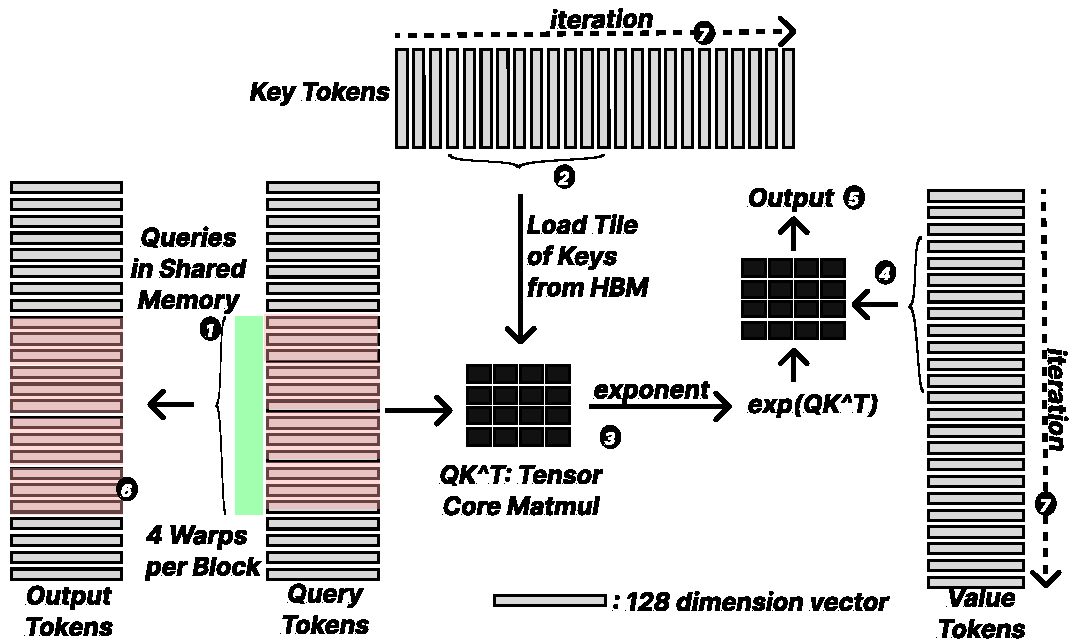
\includegraphics[width=\linewidth]{figs2/fig3.pdf}
    \caption{FlashAttention~\cite{flashattn}. Output tokens are computed by first loading a corresponding set of query tokens on chip. Then, the algorithm proceeds by iterating across all keys and corresponding values. A tile of keys and corresponding values are loaded on chip to compute attention scores, followed by exponentiation and multiplication with value tokens. }
    \label{fig:flashattention}
\end{figure}

The memory footprint when computing attention naively is $O(N^2)$, where $N$ is the sequence length.
This is the result of computing and storing $\mathbf{QK}^T$ (Eq.~\ref{eq:attn}), which requires materializing an $N\times N$ matrix for each attention head in memory. This becomes problematic when computing attention for long sequences, with the size of this intermediary $\mathbf{QK}^T$ matrix often exceeds the accelerator's HBM capacity.



Efficient implementations of attention in GPUs (flash attention~\cite{flashattn}) avoids this high memory footprint by fusing the attention score computation and the multiplication of attention map with the value matrix. This involves computing tiles of $e^{\mathbf{QK}^T}$, storing them in on-chip memory instead of HBM, and multiplying them with the value vectors. This leads to an $O(N)$ memory footprint. As a result of less memory movement in storing the intermediate matrix in HBM, flash attention is less memory-bottlenecked and achieves high SM compute utilization (and thus, is fast). 

Fig.~\ref{fig:flashattention} depicts how flash attention is mapped to a GPU kernel. The GPU kernel takes matrices for queries, keys, and values ($\mathbf{Q}, \mathbf{K}, \mathbf{V}$) as input, and produces output matrix $\mathbf{O}$. The queries, keys, values, and output tokens form a sequence of $N$ tokens (gray bars), as shown in the figure. A set of contiguous output tokens for a particular head is computed within a threadblock/cooperative thread array. The figure shows a set of output tokens highlighted in green, computed by the threads of one threadblock. This set of tokens is labeled $\mathbf{O}_{tile}$ highlighted in red.

To compute $\mathbf{O}_{tile}$, the threadblock first loads a corresponding set of queries $\mathbf{Q}_{tile}$ into shared memory~\circled{1}. Then, the first set of key and value tokens, $\mathbf{K}_{tile}$~\circled{2} and $\mathbf{V}_{tile}$~\circled{4}, is loaded into shared memory. An intermediary tile of keys/values (typically of size 64) is shown in the figure. This tile is used to compute intermediary $\mathbf{Q}_{tile}\mathbf{K}_{tile}^T$ using the tensor core~\circled{3}, followed by exponentiation to compute $e^{\mathbf{Q}_{tile}\mathbf{K}_{tile}^T}$. This intermediary result is stored in registers and is then multiplied by the corresponding $\mathbf{V}_{tile}$ using the tensor core~\circled{5}. The result of the computation is added to $\mathbf{O}_{reg}$, a slice of output in registers~\circled{6}. In the next iteration, the next tile $\mathbf{K}_{tile}, \mathbf{V}_{tile}$ in the sequence is loaded into shared memory, and computation is repeated~\circled{7}. The sum over the exponents $e^{\mathbf{Q}_{tile}\mathbf{K}_{tile}^T}$ is also computed in registers to hold the denominator of the softmax function (not shown in the figure). 





